\section{Problem definition and history}
The \emph{Travelling Salesman Problem} (TSP) is one of the most important and popular
problems in computer science. The problem consists of finding the Hamiltonian
circuit of minimum cost on a graph. The problem arose in the first half of the
20th century and it has been a key problem to develop methods and heuristics
for mathematical programming. Its resolution is very significant in practical
situations. TSP is applied in logistics, planning, and many other fields using
a slight modification of its formulation.

\begin{figure}[H] 
    \centering
    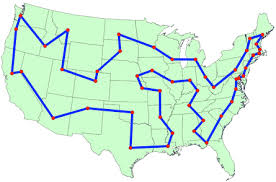
\includegraphics[width= 0.5\textwidth]{figures/tspexample.jpg} 
    \caption[TSP solved instance of USA capitals]{TSP solved instance of USA capitals}
    \label{fig:flow around cylinder} 
\end{figure} 

Travelling Salesman Problem takes its name from one of its natural application: the
the problem of a traveling salesman who has to pass through all the cities he has to
visit only once and efficiently. In a more formal description, TSP solves the following
problem: given n points and a metric function to define costs between all the pair
of node, the goal is to find a path starting and ending in the same node and passing
through all the other exactly once. To be more precise, the fact that exists a path
between every pair of nodes is a restriction of the original problem and, combined
with the fact that the distances between nodes follow the euclidean distance, we
can talk about \emph{Euclidean TSP}.

TSP belongs to the class of the NP-Hard problem and it has been for many decades
a benchmark for several innovative ideas and heuristics. For this reason,
throughout the years, the goal to solve those larger TSP instances became a
challenge for all the computer scientist. In the early 50s, the known models
could only find a solution for the problem of around 50
nodes\citep{dantzig1954solution}. In 1987 this limit grew firstly to 532 and
then to 2392. It took another 17 years to reach the goal of almost 25000 node
instances with some intermediate improvements.

\begin{table}[H] 
    \centering 
    \begin{tabular}{c|c}
        Year & Nodes \\
        1954 & 49 \\
        1971 & 64 \\
        1977 & 120 \\
        1980 & 318 \\
        1987 & 532 \\
        1987 & 2392 \\
        1994 & 7397 \\
        1998 & 13509 \\
        2004 & 24978 
    \end{tabular} 
    \caption{Solved instances milestones} 
\end{table}

For its intrinsic complexity during years a lot of approximation algorithm has
been proposed to try to achieve a good resolution in polynomial time. The first
good results in terms of approximation guaranteed a $2$-approximation solution
using a simple spanning tree technique. It has been later refined by the known
Christofides algorithm that led to a $\frac{3}{2}$-approximation using similar
ideas. However, even if it is theoretically better its results are not so
different, and being computational more demanding it is not always considered
as the best trade-off. After a very long time from these results, last year, a
paper has been presented claiming that it is possible to lower the Christofides
bound on the approximation.

\section{Mathematical Model}

If the goal aims to find the optimal solution the best know ways to do it is
using integer linear programming. TSP, in fact, can be translated into an ILP
model quite simply. The constraints ruling the model depend on the fact that
each node has to be visited and it has to be reachable from the starting one.
TSP can be formulated as a symmetric or asymmetric problem depending on the
initial requirements. The original graph-related problem, in fact, can be
expressed in both ways. However, the symmetric version of the problem can be
seen as a particular instance of the asymmetric one where from an arc two are
created having the same cost and opposite directions. For this reason, in this
introduction, we deal with the asymmetric problem.

Let now see the formal definition of the model. 

Be $G = (V, A)$ the graph for which $V$ is the set of vertices and $A$ the set
of arcs for each is defined the parameter $c_{ij},\ (i,j) \in A$ as the cost on
arc $(i,j)$.

To solve the problem new binary variables $x_{ij}$,\ $(i,j) \in A,\ i \neq j$
determines whether an arc $(i,j)$ has to be selected as being part of the tour.

\begin{equation*}
    \begin{array}{lrllr}
        \textrm{minimize}   & \displaystyle\sum_{(i, j) \in A} c_{ij}  x_{ij} \\
        \textrm{subject to} & \displaystyle\sum\limits_{(i, j) \in \delta^-(j)}  x_{ij} & = & 1 & \forall j \in V\\
                            & \displaystyle\sum\limits_{(i, j) \in \delta^+(i)}  x_{ij} & = & 1 & \forall i \in V\\
                            & \displaystyle\sum\limits_{(i, j) \in \delta^+(S)}  x_{ij} & = & 1 & \forall S \subset V : 1 \in S\\
                            & x_{ij} & \in & \{0,1\} & \forall (i,j) \in A \\
    \end{array}
\end{equation*}


The objective function aims to minimize the total cost of the solution. The
model is subject to three constraints. The first imposes that every node is
reached by an arch so it means the node is visited. The second one guarantees
that the path leaves the node so given the first constraint it means that the
path involving that node is going to be a cycle.

In the symmetric version, these two constraints can be merged into a single one
defined as
\begin{align*} 
    \sum_{(i,j) \in \delta(i)} x_{ij} & = 2 & \forall i\in V
\end{align*} 
However, even if it could seem enough, there is the need to ensure that the
model creates a single path starting and ending in the initial node. For this
reason, we impose reachability from 1 constraint, aka subtour elimination
constraint, which prevents subtours (which don't involve 1) to form. The SEC
can be also expressed in this way:
\begin{align*} 
    \sum_{(i,j) \in (S)} x_{ij} & \le |S|-1 & \forall S \subset V: |S| \ge 2,\ {1} \notin S 
\end{align*}
that explicitly express to eliminate subtours.
The formulation above is easy to write in a solver and it is correct, but it
presents a big issue. While the degree constraints are in a linear number with
respect to the number of nodes, the subtour elimination constraints in the
basic formulation are exponential and so not feasible to apply in practice. New
formulation of these constraint have made possible to deal with larger and
larger instances and in this thesis we are going to show some of these ideas
and other heuristic that made TSP feasible for significant instances.
